% !TeX root = ../main.tex

\chapter{项目简介}
\label{cha:intro}

\section{Tinker机器人的设计目标}

清华大学未来机器人团队成立于2012年,旨在帮助对机器人领域各个方面感兴趣的
同学提升技术水平,增进校内交流,提供必要的设施支持,搭建一个校内的,开放有趣的机器人
交流平台。随着团队的不断发展壮大,未来机器人团队逐渐积累了相当一批技术人才,并且开始有
机会参于国际比赛。其中Tinker机器人作为团队的主要开发项目,每年固定参加著名的RoboCup
比赛@HOME分赛场。

作为清华校内机器人方向最具影响力的学生社团,未来机器人团队在促进校内机器人相关领域的
社区发展,提高同学们的技术水平方面起到了重要影响。其中Tinker作为未来机器人团队的重要
支撑项目,在凝聚团队,提升技术水平,扩大队员眼界方面起到了重要的作用。并且Tinker本身
的技术迭代和技术积累也对校内科创发展起到了极大的推动作用,这些珍贵的技术经验不仅惠及
了未来机器人团队内部成员,也广泛的影响了校内科创领域的许多组织。

\begin{figure}
  \centering
  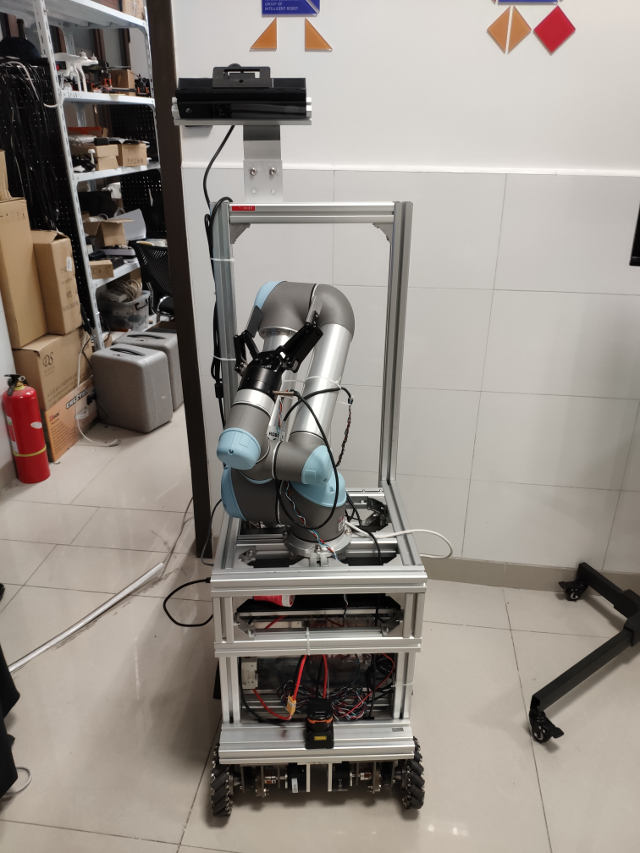
\includegraphics[width=.4\linewidth]{tinker_overview.jpg}
  \caption{Tinker外观}
  \label{fig:tinker_overview}
\end{figure}


\section{RoboCup@Home简介}

RoboCup@Home作为机器人领域的国际顶级赛事,旨在帮助提升机器人在复杂的开放环境中的表现,
促使家庭服务型机器人行业的发展。RoboCup@Home赛场分为三个联盟:Open Platform League
(OPL),Domestic Standard Platform (DSPL),Socal Standard Platform League
 (SSPL)。

三大赛事联盟中DSPL与SSPL均指定机器人的比赛,开发者不允许使用除特定机器人之外的任何机器人
参赛,且不允许替换、改装、外挂任何除机器人本身带有的部件,这两个联赛旨在促进社区内对相关
算法及软件工程的提升。其中DSPL规定使用Toyota Human Support Robot (HSR)\cite{toyota_hsr}
机器人,SSPL规定使用Softbank Robotics Pepper\cite{pandey2018mass}机器人。两款
机器人如图\ref{fig:hsr_pepper}所示。

\begin{figure}
\centering
\begin{subfigure}{.5\textwidth}
  \centering
  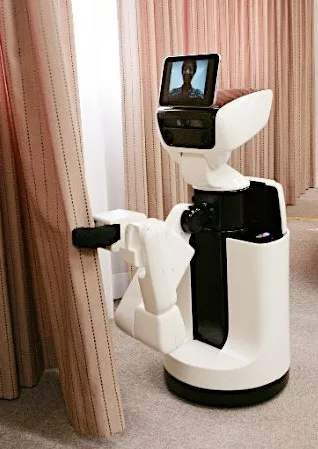
\includegraphics[width=.6\linewidth]{hsr.jpeg}
  \caption{Toyota Human Support Robot}
  \label{fig:hsr}
\end{subfigure}%
\begin{subfigure}{.5\textwidth}
  \centering
  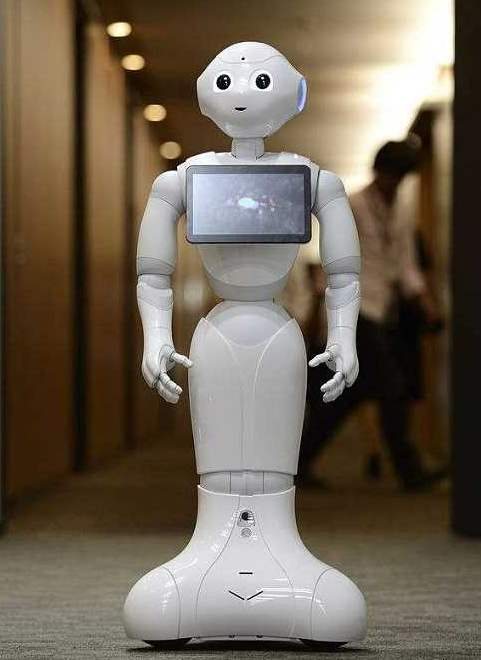
\includegraphics[width=.6\linewidth]{pepper.jpeg}
  \caption{Softbank Robotics Pepper}
  \label{fig:pepper}
\end{subfigure}
\caption{RoboCup@Home指定机器人,左HSR 右Pepper}
\label{fig:hsr_pepper}
\end{figure}

OPL为开放平台比赛,参赛者必须自行设计搭造参赛机器人,并且为机器人编写特定的软件完成比赛
中制定的任务。OPL旨在通过开放的硬件要求培养机器人领域结构、硬件相关的人才,提升各个高校
和组织中的硬件设计能力,并探索结构、硬件方面的更多可能性。Robocup@Home自2009年开始举办,
多年的比赛中OPL赛场中涌现了大量的优秀机器人设计作品,Tinker即为其中优秀的一员。除Tinker
外,还有homer@ UniKoblenz\cite{memmesheimer2017homer},Pumas\cite{savage2013pumas},
CATIE Robotics\cite{fabre2018catie}等一批外观独特,功能强大的参赛作品出现,如图
\ref{fig:other_teams}。

Robocup@Home比赛每年举行一次,举行地点在国际几大城市巡回举办,由高校或者相关组织承办。
通常比赛分为3个stage,每个stage设有若干任务,参赛队伍一次完成任务,根据完成程度和完成时
的表现(速度,流畅性等等)按点得分,分数靠前的队伍可以获得晋级资格,进入下一stage。stage I
为基础功能比赛,主要考察避障导航、抓取、识别、语音交互等基础功能,辅以合理的机器人软件控制
程序即可完成,这一个stage主要考察机器人基本的软硬件设计的自恰性及稳定性,相当多新手队伍会
在stage I直接淘汰。

stage II的任务内容同stage I基本相当,但是难度会更高,逻辑也更复杂,特别的,在近几年的比赛中,
增加了General Purpose Service Robot(GPSR),即裁判对机器人下达任意在Robocup@Home
赛场上曾经出现过的任务,考察机器人的完成情况,这一任务旨在帮助参赛者更好的构建机器人控制
软件,为家用机器人在真实场景下的应用做铺垫。

Final stage为两个得分最高的团队关于冠军奖项的争夺,每年的任务并不固定,2020年组委会
将送餐机器人作为Final Stage的考察目标,要求参赛队伍在一个嘈杂的餐厅环境中将食物托盘
送到某一个特定食客手上,并完成必要的交互。

\begin{figure}
\centering
\begin{subfigure}{.5\textwidth}
  \centering
  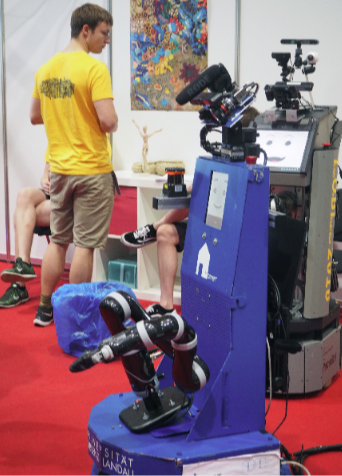
\includegraphics[width=.7\linewidth]{homer.png}
  \caption{homer@ UniKoblenz}
  \label{fig:homer}
\end{subfigure}%
\begin{subfigure}{.5\textwidth}
  \centering
  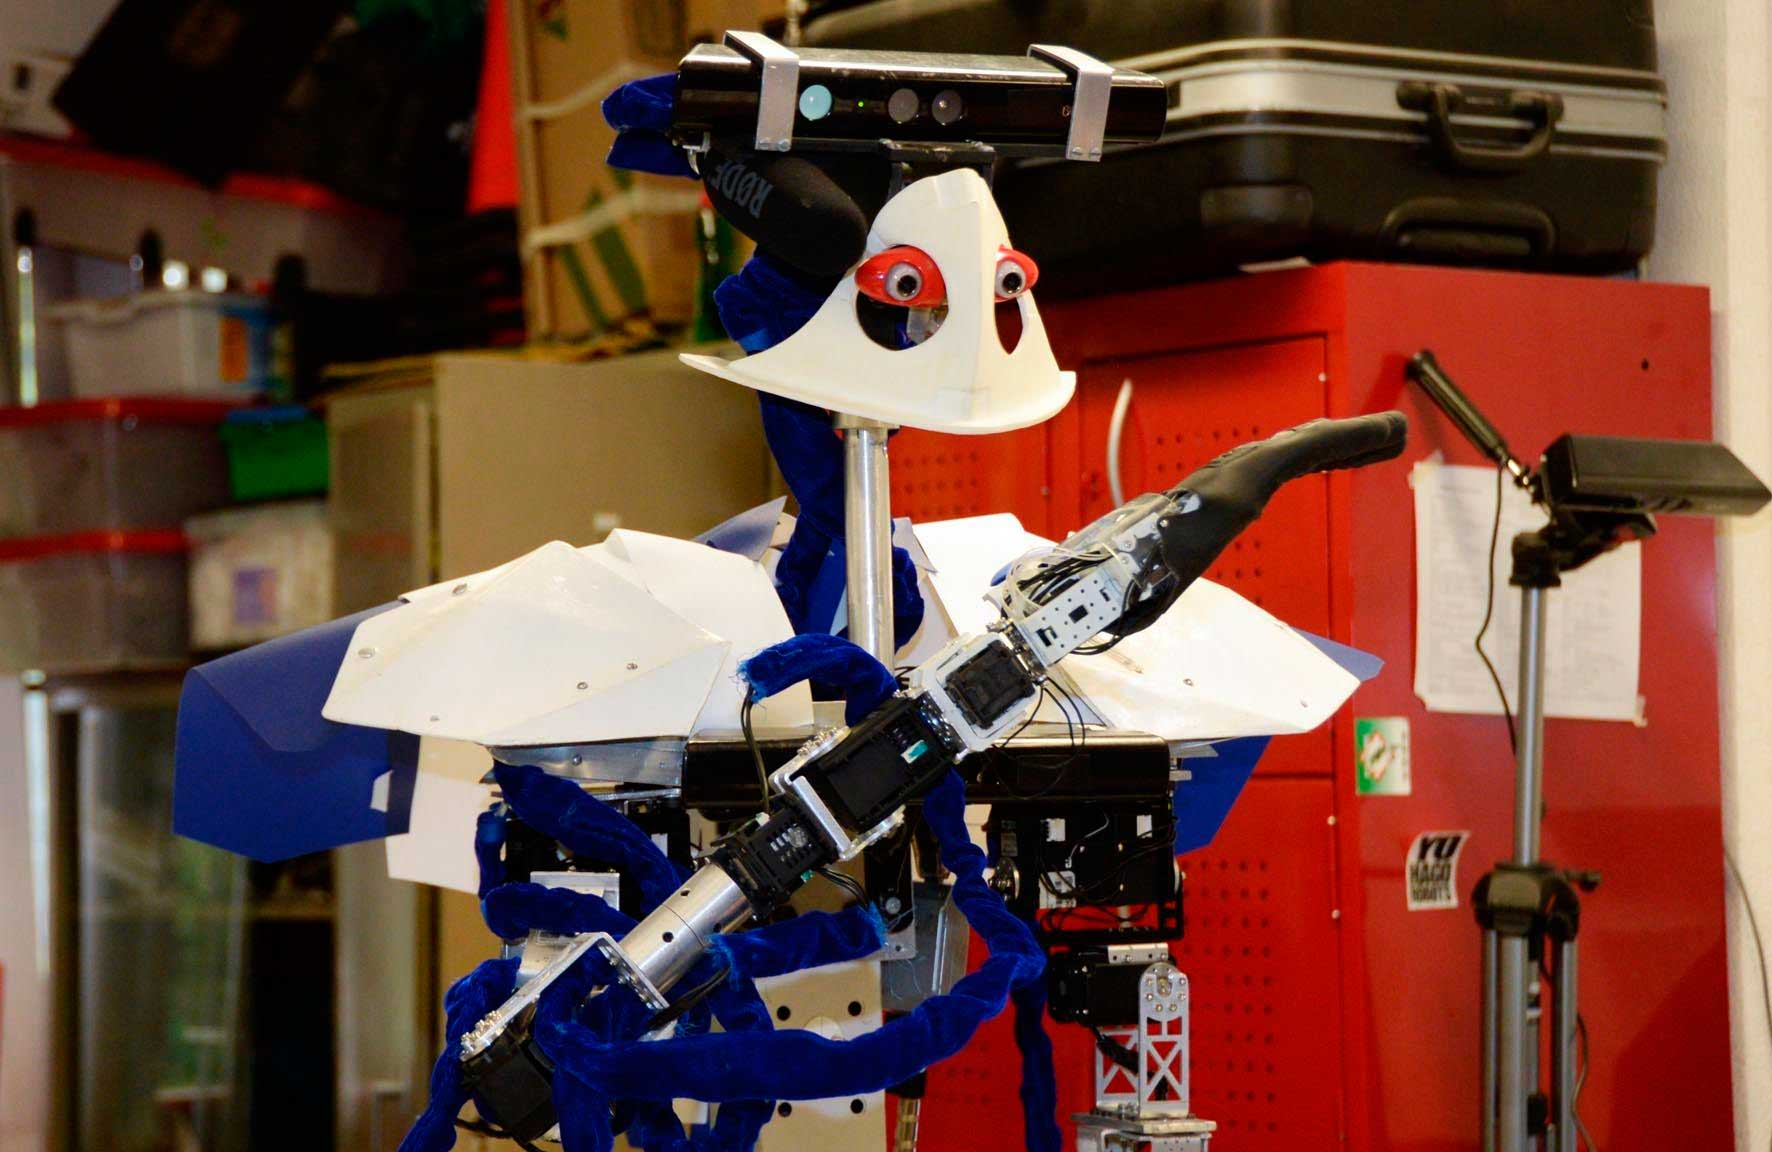
\includegraphics[width=.7\linewidth]{pumas.jpg}
  \caption{Pumas}
  \label{fig:pumas}
\end{subfigure}
\begin{subfigure}{.5\textwidth}
  \centering
  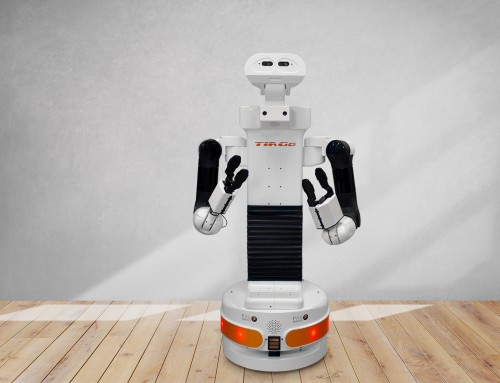
\includegraphics[width=.7\linewidth]{catie.jpg}
  \caption{CATIE Robotics}
  \label{fig:catie}
\end{subfigure}
\caption{RoboCup@Home指定机器人,左HSR 右Pepper}
\label{fig:other_teams}
\end{figure}

\section{RoboCup@Home典型任务介绍}

经过多年的发展RoboCup@Home已经培育起一个完善的社区,每年RoboCup@Home的比赛任务
即由社区相关人员协助商议决定,RoboCup@Home组委会共同维护一份RuleBook,组委会成员
使用GitHub完成RuleBook的编写任务,该仓库是完全开放且欢迎参赛者提交修改与贡献的。
RoboCup@Home组委会中,设有专门的任务制定部门Technical Committee(TC),这部分成员
大都有深厚的相关从业背景和多年的研究经验,另外有一部分成员来自各个主力参赛队伍的
核心开发人员(比如笔者作为Tinker机器人的主要程序员参与了2020年的TC工作),以
确保比赛规则同时兼顾学科研究热点和可完成性。

随着机器人行业相关技术的不断发展,RuleBook中的任务也在每年更新,并且向着越来越复杂、
越来越贴近真实生活场景的方向演进。在多年的比赛中,组委会在任务内容、任务形式上也作出
了很多改进与尝试,2019年的RoboCup@Home比赛就及其大胆的将任务数量进行了爆炸式的扩容,
尝试了很多新的复杂的任务,其中有一些被证明并不成功,因此2020年的规则制作过程中又将
不合理的任务去除,将任务数量固定为Stage I 5个,Stage II 4个。

\subsection{导航避障相关任务}

TODO


\subsection{抓取相关任务}

TODO

\subsection{识别与交互相关任务}

TODO


\section{Tinker的历史版本}

在近5年的参赛过程中,Tinker机器人经过机器人队几代同学的不断开发,经历了若干次迭代,
其硬件设计、软件架构、传感器使用、方案选择都发生了本质的变化。在Tinker不断迭代的
过程中,机器人队也积累了大量的相关经验和教训,培养出了一代代机器人相关的人才。

TODO:插Tinker之前的各种美照














